\documentclass{standalone}
\usepackage{tikz}
\usepackage{ctex,siunitx}
\setCJKmainfont{Noto Serif CJK SC}
\usepackage{tkz-euclide}
\usepackage{amsmath}
\usepackage{wasysym}
\usetikzlibrary{patterns, calc}
\usetikzlibrary {decorations.pathmorphing, decorations.pathreplacing, decorations.shapes,}
\begin{document}
\small
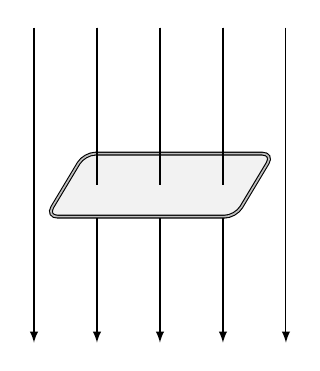
\begin{tikzpicture}[>=latex,scale=0.8]
  \useasboundingbox(0.9,0)rectangle(5.1,5);
  \foreach \x in {1,2,...,5}
  {
      \draw[->](\x, 5)--(\x, 0);
  }
  \draw [double=lightgray,rounded corners,fill=lightgray!20](1.8,3)--(4.8,3)--(4.2,2)--(1.2,2)--cycle;
  \foreach \x in {2,3,4}
  {
      \draw(\x, 5)--(\x, 2.5);
  }
\end{tikzpicture}
\end{document}